\section{Binære søketrær}
\label{bintraer}
Binære søketrær er trær med noen spesielle krav. Hver node kan ikke ha mer enn to barn, vi kaller dem ofte venstre og høyre barn. Venstre barn er alltid mindre enn noden selv, og høyre barn er alltid større enn noden. Dette gjør binære søketrær meget godt egnet for søking. 

\begin{theorem}
\label{teo:bintre}
Å sette inn, fjerne eller søke etter noder i et binært søketre har
\begin{enumerate}[i]
\item I beste fall $ O(\log n) $ tid
\item I verste fall $ O(n) $ tid
\end{enumerate}
\end{theorem}

Vi skal ikke bevise teorem \ref{teo:bintre} her\footnote{Det kan vises ved induksjon at høyden til et binært tre i beste fall er $ \log_2 n $}, men vi kan se på et eksempel som viser ytterpunktene. I figur \ref{fig:bintre} ser vi to forskjellige binære søketrær. I treet til venstre har vi et fint, balansert tre. Det er lett å se at høyden (og dermed antall operasjoner vi må gjøre for å komme til bunn i treet) er lik $ \lceil \log_2 n \rceil $ der $ n $ er antall noder i treet.

I treet til høyre har hver node kun ett barn. Vi har i praksis en lenkeliste. Hvis vi skal søke etter 4, må vi tråkke gjennom alle de andre nodene for å komme dit. 

\begin{figure}[h!tb]
\caption{To eksempler på binære søketrær}
\label{fig:bintre}
\centering
~\\
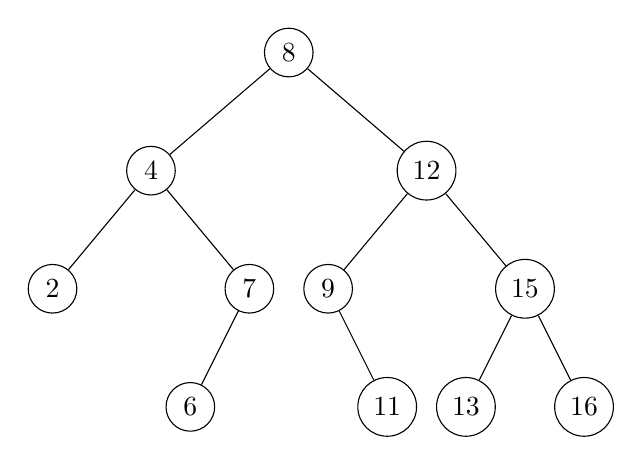
\begin{tikzpicture}[level distance=1.5cm,
  level 1/.style={sibling distance=3.5cm},
  level 2/.style={sibling distance=2.5cm},
  level 3/.style={sibling distance=1.5cm},
every node/.style = {shape=circle, draw, align=center}]

\node{8}
	child {node {4}
		child {node {2}}
		child {node {7}
			child {node {6}}
			child [missing]{}
		}
	}
	child {node {12}
		child {node {9}
			child [missing]{}
			child {node {11}}
		}
		child {node {15}
			child {node {13}}
			child {node {16}}
		}
	};
\end{tikzpicture}
$ \quad\quad $
\begin{tikzpicture}[level distance=1.5cm,sibling distance=2cm,
every node/.style = {shape=circle, draw, align=center}]

\node{1}
	child [missing] {}
	child {node {2}
		child [missing]{}
		child {node {3}
			child [missing]{}
			child {node {4}}
		}
	};
\end{tikzpicture}
\end{figure}




\subsection{Innsetting}
Når vi skal sette inn en node i et binært søketre starter vi i rota. Vi sammenligner verdien vi skal sette inn med verdien i rota. Hvis verdien vi setter inn er mindre enn rota går vil til venstre, er den større går vi til høyre. Hva som skjer ved likhet er opp til oss å bestemme, men vi må være konsekvente. Når vi kommer til en nullpeker kan vi sette denne pekeren til å peke på noden vi setter inn.

Vi kan implementere denne funksjonen rekursivt. I en ytre klasse kan vi skrive en skallfunksjon som kaller på rotas \mono{insert}-metode. Vi har en indre \mono{Node}-klasse med en rekursiv insertmetode. Den kan implementeres slik:
\javaimport{code/ex_bintree_insert.java}


\subsection{Sletting}
Når vi skal fjerne en node fra et binært søketre har vi tre forskjellige situasjoner som vi må se på.

{\bfseries Noden har ingen barn} (løvnode). Denne situasjonen er ganske grei. Siden noden ikke har noen barn å forholde seg til er det bare å fjerne den fra treet.

{\bfseries Noden har ett barn}. For å fjerne en node $ a $ med ett barn kan vi ganske enkelt flytte pekeren fra foreldernoden til $ a $, til barnet til $ a $.

{\bfseries Noden har to barn}. Hvis noden vi skal fjerne har to barn tar vi opp den minste noden som er større en noden vi skal fjerne og flytter den til den posisjonen noden vi skulle fjærne var. Vi finner den minste noden som er større ved å gå ett steg til høyre, og så til venstre helt til vi er i bunn av treet. 

Eksempel på implementasjon i Java (rekursiv metode i en \mono{Node}-klasse):
\newpage\javaimport{code/ex_bintree_remove.java}

\vspace{-6pt}
\subsection{Søking}
Når vi skal søke etter et element i et søketre starter vi i rota og sammenligner det elementet vi søker etter med det elementet som finnes i rota. Er elementet vår mindre enn noden vi ser på går vi til venstre, og er det større går vi til høyre. Deretter foretar vi samme testen på nytt og fortsetter slik til vi enten finner elementet vi leter etter, eller kommer til en nullpeker (bunnen av treet).

Eksempel på implementasjon i Java:
\javaimport{code/ex_bintree_search.java}